\chapter{项目背景}
% \label{cha:intro}
\label{cha:background}


\section{社会背景}
法律是治国之重器,表明了国家权力的运行和国家意志的体现。法律在规范个人、保障社会秩序方面起到了非常重要的作用,同时法律也是我们每一个人维护自身权益的保证。因此,法律对于国家、社会、个人都是相当重要的。自新中国成立以来,全国上下各个司法机构、学术领域产生了大量的法律文书、法学期刊等文件。这些法学文件一直以来被法学领域的学者、法官、律师重视,成为了他们工作中非常重要的一个部分。自国家全面推行依法治国以来,法律在我们日常生活中扮演着越来越重要的角色。但是,当人们在生活中遇到法律问题时,却常常因为缺乏专业知识而不知道如何进行维权。同时,法学领域的学者、工作人员在面对浩如烟海的法律文本时,也常常因为缺乏好的检索工具和阅读系统,而需要花费大量的时间来查找相关材料,大大降低了工作效率。目前我国司法建设面临着严重的考验。

\textbf{案多人少形势严峻}。近几年来,中国每天发生的法律案件日益增加,据统计,2018年人民法院受理的案件高达2800万件,创下历史新高。每年案件数量依旧以14.5\%的速度进行增长,然而中国法官数量相比2012年却减少了40\%,这带给众多一线法官巨大的工作压力。案多人少的严峻局面给国家的司法公平公正提出了巨大的挑战。据数据统计,2018年平均每个法官一年审理案件高达233件,是2008年的\textbf{4倍}。然而法律领域对人才的严苛性让法官数量的增加受到很大的限制。

\begin{figure*}[ht]
    \centering
    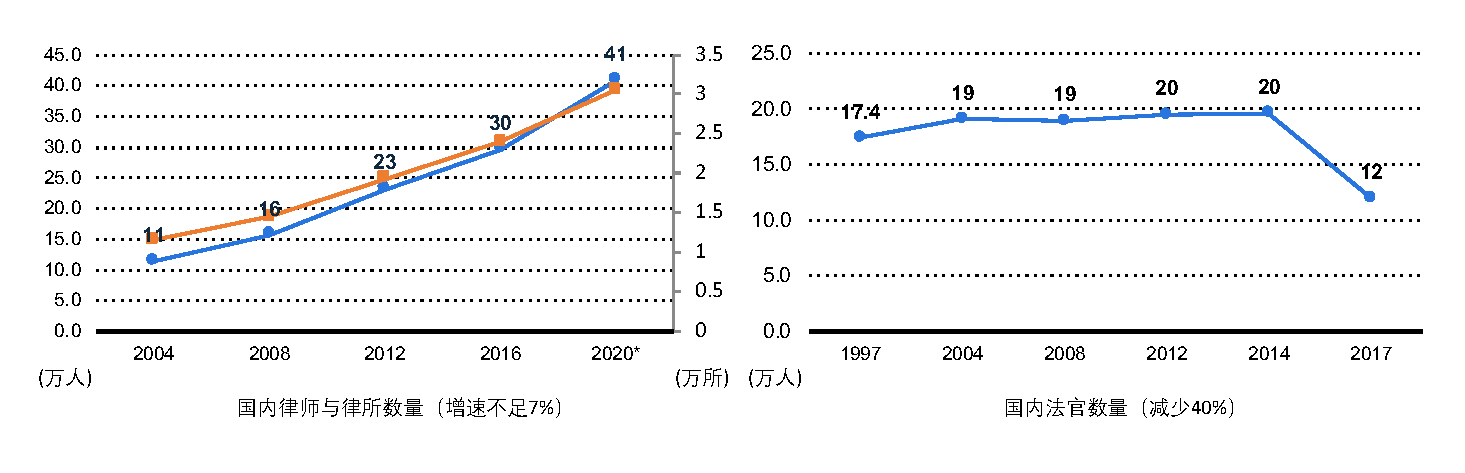
\includegraphics[width=\linewidth]{figures/professional_num}
    \caption{中国法学专业人士数量}
    \label{fig:professional_num}
\end{figure*}

\begin{figure*}[ht]
    \centering
    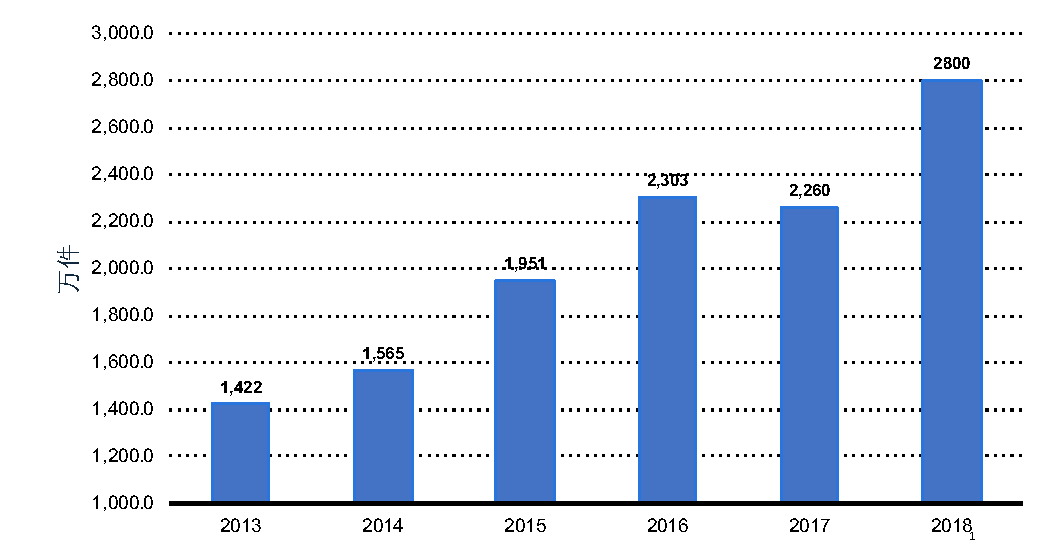
\includegraphics[width=\linewidth]{figures/case_num}
    \caption{中国法院受理案件数量(增速达\textbf{$14.5\%$})}
    \label{fig:case_num}
\end{figure*}

\textbf{法律服务需求缺口巨大。}目前,我国发生的案件中有80\%无法得到专业律师代理。与此相反,在美国人均律师数量是中国的15.6倍。同时我国律师地区分布也具有极大的差异性,80\%的律师集中在中国20\%的城市,这也就表明偏远地区人民在获取法律服务时更是难上加难。这些数据表明,法律服务在中国具有庞大的市场规模,但是由于人才供应不足,大多数人在遇到法律问题时,有求而无应。

\textbf{大量司法数据的累积。}自从国家立法以来,全国上下各级法院产生了大量的司法文件。得益于司法公开化进程推进,国家已经公开了超过6千万的法律案件文书、数千部法律与司法解释,同时,在众多的法学学者努力下创办了几百种权威的法学期刊。这为人工智能介入司法领域提供了数据基础。

\textbf{技术的高速发展。}目前,技术的创新给我们的生活带来了许许多多的改变,其中表现最突出的便是人工智能与大数据的技术。伴随着深度学习的发展,人工智能中的许多领域在近几年来取得了很大的进步。自然语言处理技术便是其中的代表,在该领域中文本分类、知识图谱、信息抽取、机器翻译等任务上,现有模型纷纷打破了前人的纪录。技术的创新带来的是生活的改变,而这样的改变也逐渐渗透到法学领域。2018年,司法部提出“加快‘数字法治、智慧司法’建设”的口号 ,这也让法学学者也越发注重人工智能在司法领域的应用。


\section{商业背景}
随着司法公开化进程的不断推进,目前市面上涌现了许多与法律服务有关的工具、平台。现有平台大多作为一个数据库检索工具,为法律工作者提供了较多的底层基础服务。经过许多年各大数据库之间的竞争与互相学习,各大数据库之间的数据与检索手段大同小异。我们将介绍目前主流平台提供的主要的法律服务:
\begin{enumerate}[1)]
	\item 案件文书、法律法规关键词检索。近几年不断涌现的法律服务平台均将案件文书、法律法规检索作为平台功能的核心。这些平台大多利用传统统计算法,获取输入关键词,计算词语匹配信息来推荐相关的文书与法条。基于关键词的检索,常常因为需要大量的背景知识来对事实进行凝练而无法普及。并且,词语匹配的检索也将受到高频无关词语的影响,而无法进行长文本检索。
	\item 法律咨询问答。许多平台意识到基于关键词的案件检索对于普通民众具有较高的知识门槛。因此为了拓宽平台受众面,许多平台纷纷与律师事务所合作,提供了法律咨询问答的服务。这些问题与“百度知道”等网络社区类似,提问者提出问题后,为回答问题者提供回馈,以吸引专业人士回答。但是这样的咨询社区因为律师数量有限、反馈不及时,同样无法提供很好的解决法律问题。
	\item 法律知识获取。为了帮助法学工作者更好获取相关知识,许多平台提供了法学期刊论文检索、书籍内容检索。这些内容以法律专业术语构成,可以帮助法学学者更好地阅读相关工作,但对于大多数人而言,该模块并无法很好帮助他们解决法律问题。
\end{enumerate}
~\\

上述功能在一定程度上能够帮助法学工作者提供相应的专业帮助,却因为功能单一、效率低而无法得到普及。即,平台提供的功能依旧无法很好帮助生活中每一个人解决法律问题。我们总结了如下现有平台面临的缺陷:
\begin{enumerate}[1)]
	\item 使用门槛高,受众范围小。基于关键词的检索,需要用户从事实中精简、总结出相关的法律专业术语,并从搜索引擎返回的结果中,利用背景知识进行筛选、重排序出对现有事实有意义的法律文书。这些操作需要很多的背景知识,这也就意味着现有平台无法面向普通人提供法律服务,这也是目前即使市面上涌现了这么多法律产品却无法为普通人提供及时、专业的法律援助的重要原因。
	\item 无法支持语义检索。目前市面上的法律服务平台采用的是传统的统计模型,即使可以支持精确检索与模糊检索,却依旧受到多个因素干扰。基于词语匹配的算法只能检索文本类似的案件文书。然而案件事实描述是一个具有很大多样性的文本,无法捕捉语义意味着检索结果具有很大的偏差。例如,检索词语“打架”,从语义角度理解,应该检索具有打架事件的事实(包括打斗、争执等词语),但是传统平台只会检索包含“打架”一词的文本。这很大程度上,限制了检索的效果。
	\item 功能单一,无法分析长文本案件。长文本检索一直以来,受到无关词语干扰重排序结果的影响,而无法很好的推广。然而对于普通人而言,长文本案情分析是非常重要的功能之一,可以降低平台使用门槛,同时尽可能多捕捉案件信息,帮助大家解决法律问题。
\end{enumerate}
~\\
因此,为了解决以上问题,团队提出了一个面向普通人的案情分析平台JudgeAI,平台从多个角度对案件进行预测分析,实现了零门槛。表格\ref{background:compare}对比了JudgeAI平台与市面上常用的法律服务产品的功能,可以发现JudageAI具有最全的功能,最低的使用门槛。

% 根据团队调研结果,市场上的产品可以大致分成两类:以搜索引擎为主体的法律文书检索系统、以检索的技术为主的问答系统。接下来我们将分别介绍这样两类系统及其代表,并简要阐述其缺点。

%文书检索系统是市面上出现最早的、目前应用也最广泛的法律应用。自从国家启动司法案例公开化之后,裁判文书网 便成为了拥有文书数量最多的官方平台,但是由于其检索速度慢、检索结果不全而没有成为一个使用广泛的工具。随后,许多其他检索工具(如无讼 、北大法宝 等)应运而生,相对于裁判文书网,这些网站增加了法律法条、指导案例的检索功能,但由于其采用的仍是基于词语匹配的检索算法,这些检索工具依旧无法从语义角度进行内容的检索,这样一个缺点在进行长文本检索时尤其突出。我们以北大法宝检索为例,在检索转化型抢劫的一般情形——“偷窃被发现,用暴力导致被害人受伤”时,北大法宝并未返回相关结果。因此,目前市场上的搜索引擎以词语匹配为技术手段,无法很好的服务于大众。

%另一类市场上较多的法律产品是以检索技术为主的问答系统。问答是自然语言处理中的热门问题,但因为效果原因并未有很好的应用,而现有产品将问题进一步简化。例如京东推出的一款名为“法咚咚”的问答产品,通过将问题限定领域,并利用现有的检索技术,在用户输入问题时,通过词语匹配技术来推荐相关的法律依据。技术的限制也让这样一个产品有了许多限制:无法分析实际情景、使用者需要有法律背景。同期搜狗提出的“搜狗律师”也面临着同样的问题。% 随着法律智能受到社会的广泛关注,各大有关公司也都推出了相应的产品。其中最具代表性的法律工具网站有:中国裁判文书网、北大法宝、法信网、法咚咚、搜狗法律等。这些产品大多以基于词匹配的案件文书检索为核心。受限于统计方法的检索能力,这些产品大多面向法律专业人士,旨在为他们提供基础的法律服务。

\begin{table}[ht]
\begin{tabular}{c|ccccc}
\hline
评价指标             & 语义检索       & 关键词标签      & 法学要素       & 案情分析预测     & 长文本检索      \\ \hline
裁判文书网            & ×          & ×          & ×          & ×          & ×          \\
北大法宝             & ×          & √          & ×          & ×          & ×          \\
威科先行             & ×          & ×          & ×          & ×          & ×          \\
无讼               & ×          & √          & ×          & ×          & ×          \\ \hline
\textbf{JudgeAI} & \textbf{√} & \textbf{√} & \textbf{√} & \textbf{√} & \textbf{√} \\
\hline
\end{tabular}
\caption{JudgeAI与市面上常用产品对比}
\label{background:compare}
\end{table}

\section{项目难点}
人工智能技术经过几十年的不断发展,已经取得了很大的进步与突破。近今年,深度学习技术受到越来越多学者的追捧,深度神经网络模型凭借着强大的自动抽取特征的能力在许多任务上超越了人类表现。同时,伴随着近几十年海量数据的不断累积、硬件高速发展带来的强大算力,神经网络已经渗透到我们生活的各个领域,并利用它强大的特征自动抽取能力,在效果上超过了传统机器学习算法,从而受到商业界、学术界的认同。但是,随着学者研究的不断深入,深度学习也逐渐暴露出其难以避免的缺点,这也给深度学习进入智慧司法领域带来了许多的困难。
\begin{itemize}
	\item \textbf{模型不可解释性}。在深度学习系统中,分类器和特征模块都是自动学习的,神经网络就有了一个灰色区域:可解释性问题。而深度学习系统这样一个“黑箱”性质一直被学者们诟病。缺乏数学公式推导,给定输入,我们无法获知模型将如何产出结果,无法获知模型为何会产生这种结果。尤其是在多任务学习的深度学习系统中,系统常常产生互相矛盾的预测结果。然而在法律智能领域,模型可解释性将是极其重要的一点,任何司法问题都需要有严格的法条文本支撑、需要有严密的推理逻辑支撑。这也是自然语言处理技术发展迅速却无法在法律智能实用系统中起作用的重要原因之一。
	
	\item \textbf{知识理解差、推理能力差}。如何让深度学习系统理解知识并运用到相应的任务中一直是许多学者的目标。近几年,为了发掘深度学习系统在理解文本语义上的能力,许多学者提出了不同的阅读理解数据集\cite{nguyen2016ms,rajpurkar2016squad,trischler2016newsqa},希望能够检验模型在文本阅读、理解上的能力。通过许多年的努力,许多深度学习模型在这些数据集上的表现已经超过人类。但是模型其实并未理解文本语义,而只是有较强的文本对比匹配能力\cite{clark2018think}。\citet{kwiatkowski2019natural}实验表明,神经网络系统在需要推理的文本理解问题上表现不佳。在法律领域,如何理解海量的法律知识,并将其运用至实际生活中,是法律智能领域落地重要技术难题。
	
	\item \textbf{少样本学习}。深度学习模型早在上个世纪便被提出,然而却并没有收到学者关注,直到2012年,\citet{krizhevsky2012imagenet}将深度学习模型运用到ImageNet图片分类中,随之深度学习模型引起了人工智能领域学者的广泛关注。而之所以深度学习模型直到30年后才被发现其价值,最主要原因便是深度学习需要大规模数据训练,而上个世纪互联网没有普及,数据收集极其困难。直到现在,深度学习依旧因为“数据饥饿”的性质而受到许多的限制,少样本学习也成为许多学者关注的重点。在智慧司法领域,即使拥有数千万的法律文书,我们依旧面对着严重的数据不均衡导致的样本缺少的问题。据数据统计,刑事案件中高频的十类案件占总案件数量78.1\%,而低频的50个罪名,只占总案件数量的不足0.5\%。这也成为了法律智能系统不得不解决的重要问题。
	
\end{itemize}
~\\
通过长时间努力,团队针对以上难点,提出了相应的解决方案,一定程度上克服并解决了上述难点给智慧司法技术落地带来的苦难。
\\

在这样的契机之下,团队构建了一个案情分析平台——JudgeAI,尝试将自然语言技术运用到法学领域的各个问题之上,旨在利用自然语言处理的技术的方法来解决实际法律问题,为大家的工作、生活提供便利。我们实现了对案情的全方面多角度的分析,在输入一段文本形式案情描述之后,我们平台将提供:案件的案由/罪名预测、判案要素预测、相关法条预测、相似案件检索、关键词提取和相关问题推荐的功能。以此让用户能够尽快捕捉到文本中的有用信息,并作出相应的判断,从而达到辅助判决的作用。相比于已有的产品、算法,我们团队在这些任务上提升了对长文本语义的理解,超过以往模型,达到了更高的预测精度。
